\section{Proposed Method: \method}\label{sec:proposal}

The method proposed by \method organizes the generation of a preliminary sewer network into three moments: data preparation, graph processing, and serialization of the resulting network. The process starts from an urban area selected by the user, from which the system obtains public street data, enriches vertices with elevation, builds an editable graph, and allows manual adjustments before processing.

\subsection{Data preparation}

During data preparation, urban streets are obtained from OpenStreetMap through queries to the Overpass API and represented as GeoJSON \cite{osm2026}.
Topography is obtained through the OpenTopography API, which returns digital elevation models in GeoTIFF format \cite{opentopography2026}.
The system samples elevation values at street vertices, handles missing values or border artifacts, and keeps elevation attributes associated with graph nodes.
This step transforms raw geographic data into a structure that can be manipulated by the editor and by the backend.
Figure~\ref{fig:area-selection} illustrates the first interaction of this flow, in which the user defines a bounding box over the map and the system checks the selected area before fetching geospatial data.

\begin{figure}[H]
\centering
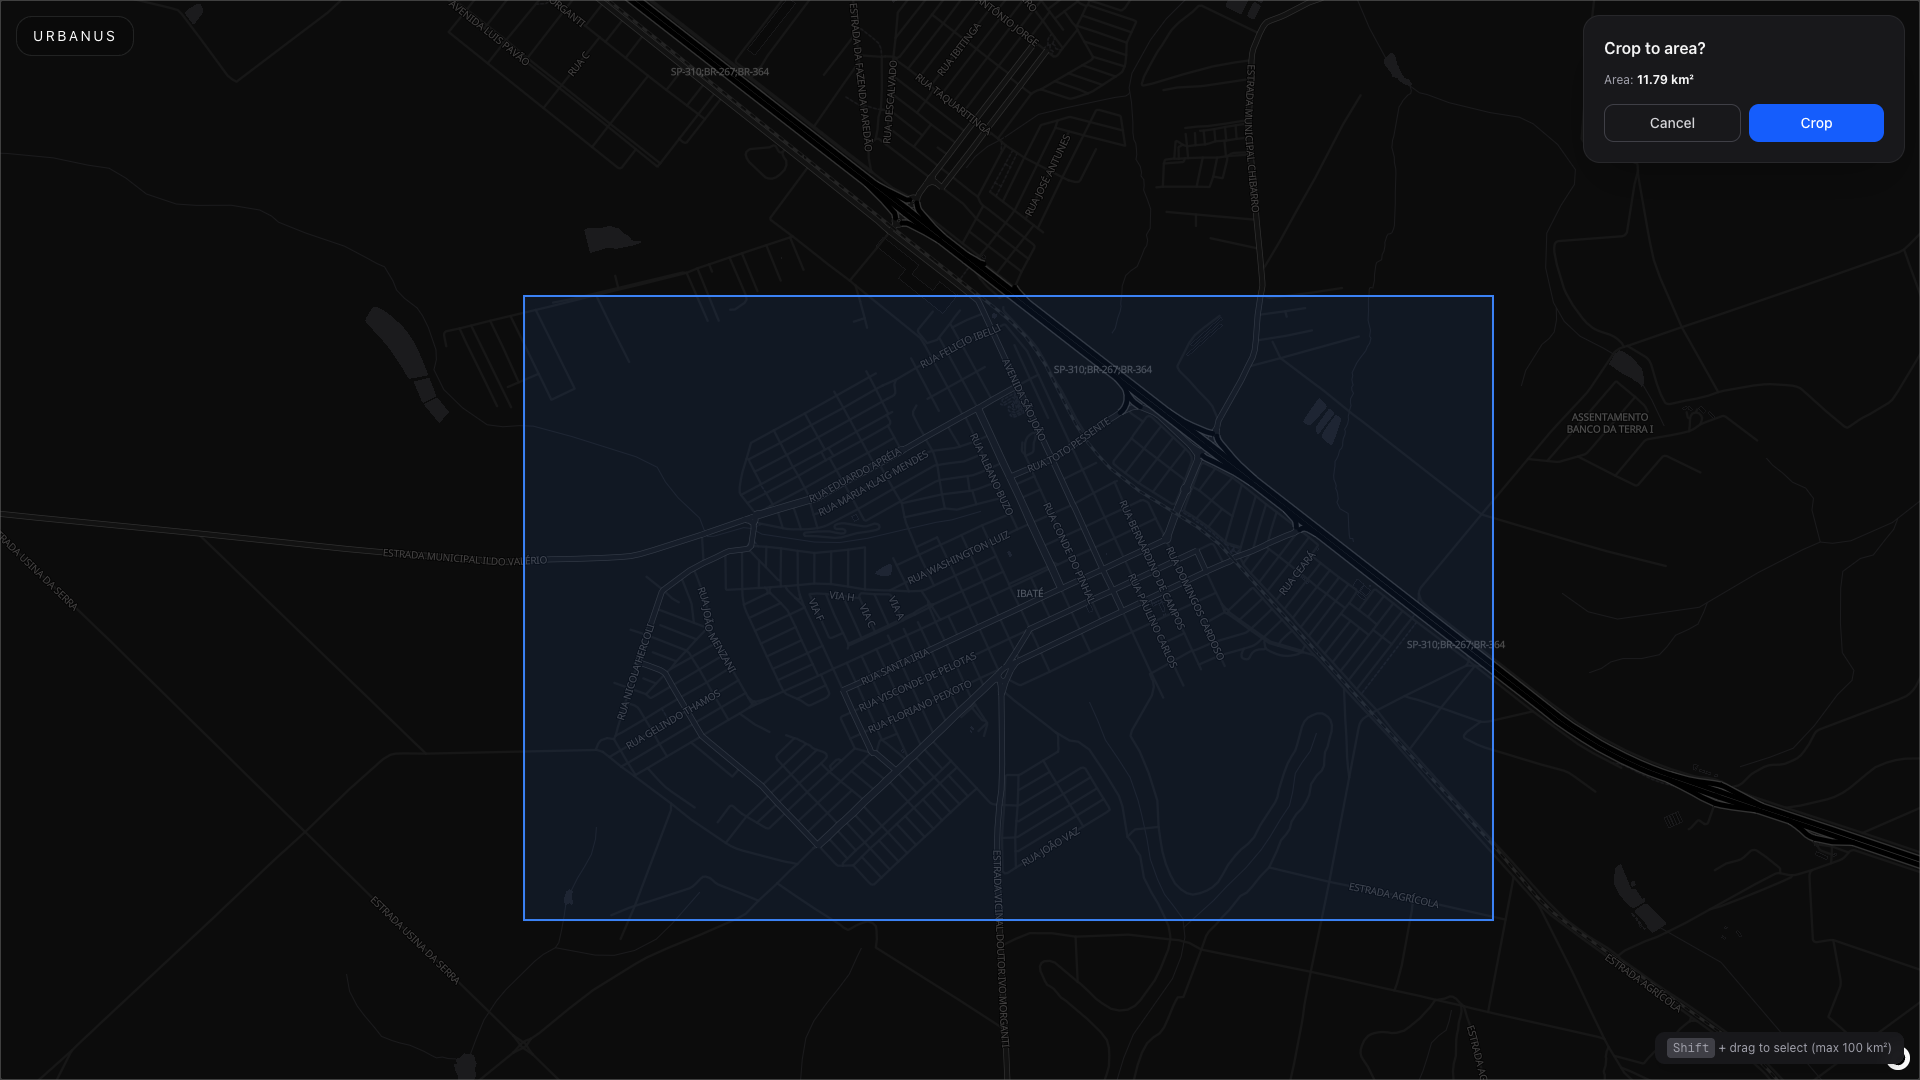
\includegraphics[width=.95\linewidth]{images/bounding-box-draw.png}
\caption{Area-selection step used to define the region processed by \method.}
\label{fig:area-selection}
\end{figure}

\subsection{Edited graph as processing input}

Before processing, the user can inspect and edit the graph.
This decision is methodologically important because the current system does not depend on an automatic reconstruction from the original GeoJSON after the user has made changes.
The edited graph becomes the source of truth for the pipeline.
Thus, the backend processes exactly the structure that the user visualized and adjusted, reducing the possibility of divergence between the interface and the computed network.
Figure~\ref{fig:graph-views} shows two complementary editor views of the same project: one emphasizing road categories and another emphasizing elevation values sampled along the graph.

\begin{figure}[H]
\centering
\begin{minipage}{.49\linewidth}
\centering
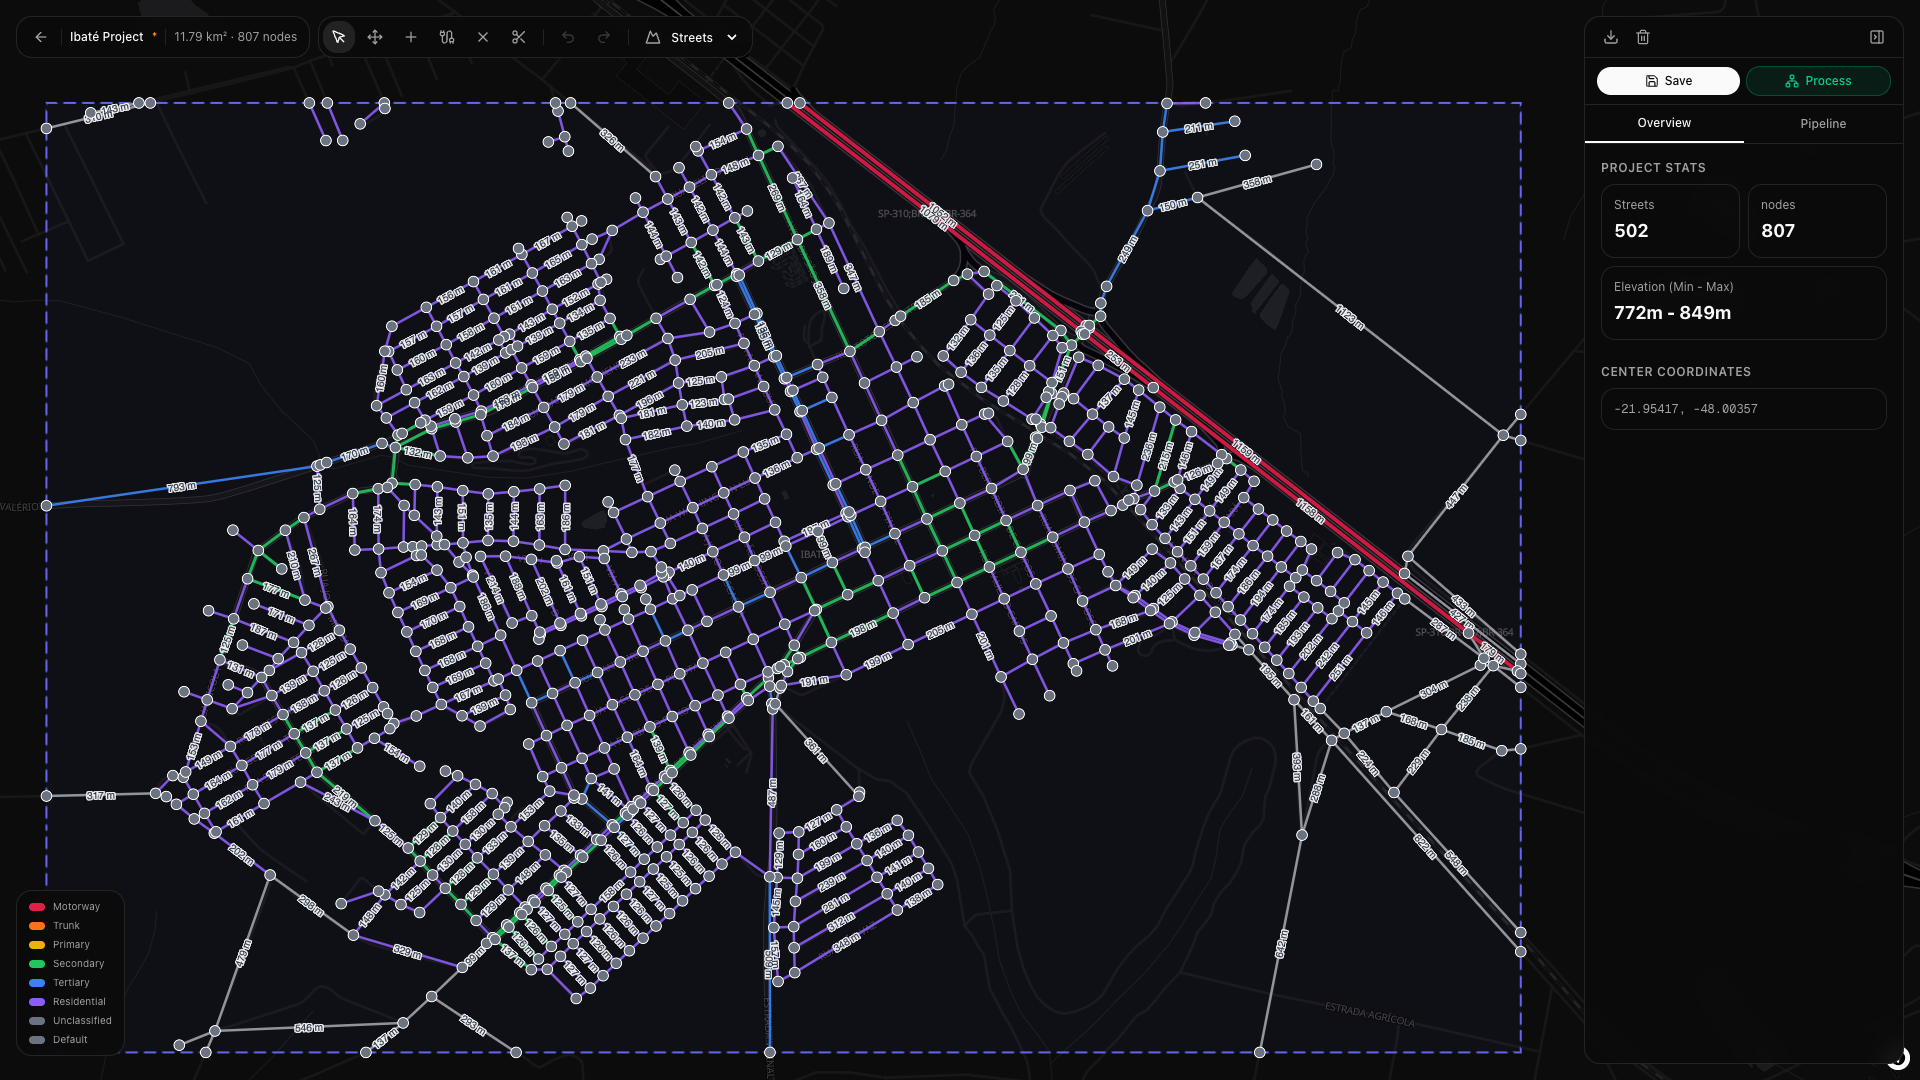
\includegraphics[width=\linewidth]{images/map-view-streets.png}
\end{minipage}
\hfill
\begin{minipage}{.49\linewidth}
\centering
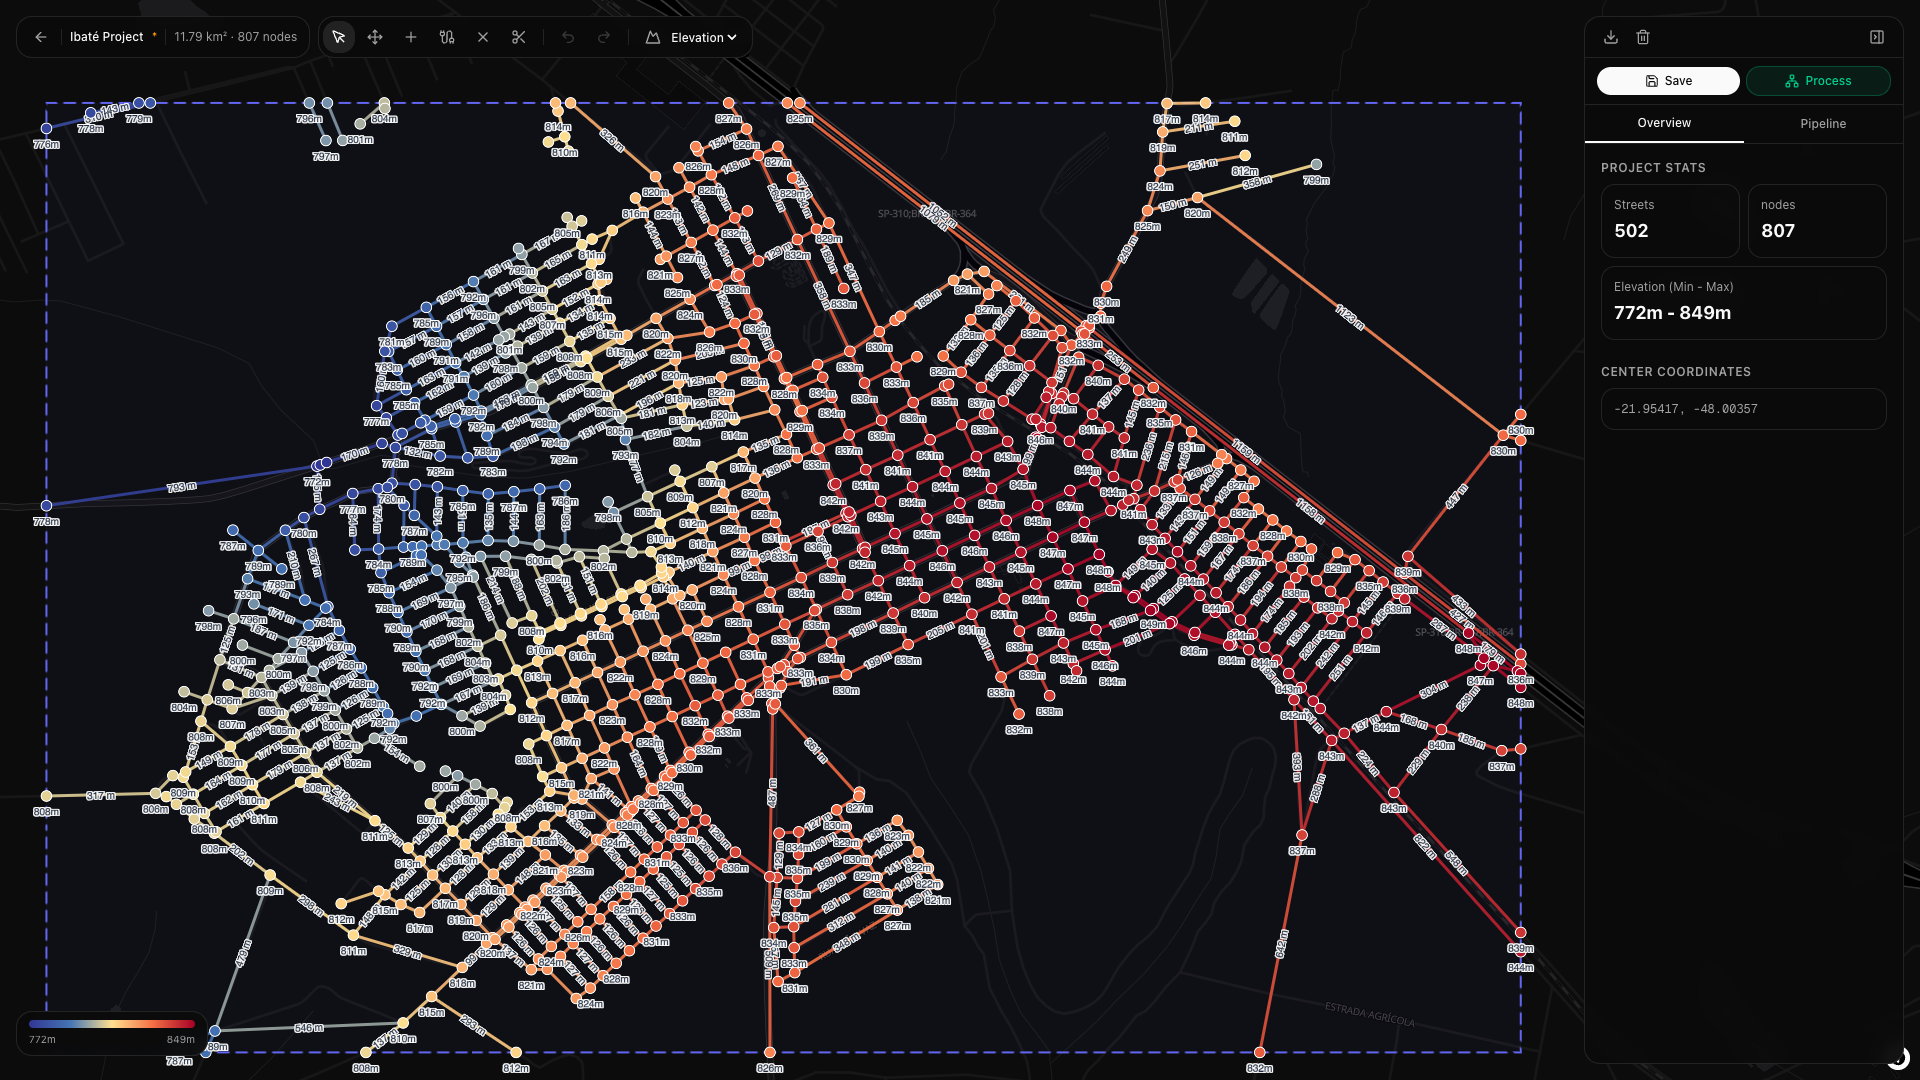
\includegraphics[width=\linewidth]{images/map-view-elevation.png}
\end{minipage}
\caption{Editable graph views: road-category visualization on the left and elevation visualization on the right.}
\label{fig:graph-views}
\end{figure}

\subsection{Graph processing pipeline}

Processing starts by reconstructing the graph in NetworkX.
Then, the system applies safeguards over elevation data, identifies mandatory nodes, marks direction changes, removes redundant nodes, and applies spacing rules between manholes.
It then detects local maxima and minima, identifies grade breaks, and selects collection points.
These steps prepare the graph for routing by preserving relevant elements of the mesh and reducing points that do not contribute to network interpretation.

Gravitational routing uses the Repeated Shortest Path Heuristic (RSPH) to connect mandatory nodes and collection points to an outlet or to local collectors.
The heuristic performs successive least-cost path searches, updates the network under construction, and favors the reuse of trunks.
After routing, the pipeline repairs missing edge coverage, removes cycles when necessary, optimizes the position and quantity of nodes, and assigns inspection accessories to the remaining physical nodes.
The output is a serialized preliminary network with nodes, edges, lengths, slopes, elevations, flow directions, and relevant point markers.
Figure~\ref{fig:rsph-routing} details the routed network after processing, including flow-direction arrows and collection-point markers used to inspect the generated solution.

\begin{figure}[H]
\centering

\includegraphics[width=.78\linewidth]{images/view-of-rsph-routing-to-collection-point.png}
\caption{Detailed view of the processed network, highlighting RSPH routing, flow direction, and collection points.}
\label{fig:rsph-routing}
\end{figure}

\subsection{Architecture and implementation}

The system is organized as a polyglot monorepo.
The JavaScript/TypeScript part uses a pnpm workspace, while the Python part uses a uv workspace.
This organization keeps related applications and packages in the same repository, separating responsibilities without duplicating domain concepts.

The frontend was developed with Next.js, React, TypeScript, Tailwind CSS, MapLibre, React Map GL, Zustand, and React Query.
The interface includes map area selection, street import, interactive graph editing, visualization controls, editing state, result panels, and alternation between the original mesh and the processed network.
The editor supports node selection, movement, creation, connection, splitting, and removal, as well as undo and redo actions.

The backend was developed in Python with FastAPI, Pydantic, SQLAlchemy, GeoAlchemy2, Shapely, Rasterio, NumPy, httpx, and NetworkX.
FastAPI exposes routes for project creation, listing, reading, and deletion, as well as routes for node extraction, elevation enrichment, and network processing.
NetworkX is used as the graph structure for algorithmic steps, while PostGIS provides geospatial persistence.

Projects are persisted in PostgreSQL with the PostGIS extension.
The database stores metadata, selected area, map center, statistics, street GeoJSON, and the processed network.
Node and edge tables store spatial geometries and attributes such as elevation, node type, length, slope, and auxiliary properties.
Thus, the processed result can be saved, reloaded, and inspected later.

Shared TypeScript packages were also created for geographic types, constants, and utilities, together with a Python package containing Pydantic types and geographic calculations.
This division follows the principle of sharing contracts, not implementations: each ecosystem keeps its own implementation, while the central concepts remain aligned through types, constants, and parity tests.
